% Ubah judul dan label berikut sesuai dengan yang diinginkan.
\section{Experiment}
\label{sec:experiment}

% Ubah paragraf-paragraf pada bagian ini sesuai dengan yang diinginkan.
Containing in this section we will explaining the result of our test along with the analysis that we have been in accordance with the system design written at the previous section. Dataset that is being used is a combination of dataset that is originated from \url{data.mendeley.com} and dataset of our own creation by leveraging web crawling technology. There are a few experiment that we have run in this research with details summarize as below :

\begin{enumerate}[nolistsep]
  \item Performance experiment based on the text truncating method
  \item Performance experiment based on the BERT model that is being used
  \item Performance experiment based on the transformer method being used
  \item Performance experiment based on the training approach
\end{enumerate}

In each of these experiment, all of the models is ran on Google Collab with hardware specification enlisted in table \ref{tab:specs_collab}

\begin{table}[h]
  \caption{PC specification that we use}
  \label{tab:specs_collab}
  \centering
  \begin{tabular}{|l|l|}
    \hline
    \textbf{Processor}            & 2 v-core Intel(R) Xeon(R) CPU @ 2.20GHz   \\ \hline
    \textbf{RAM}                  & Virtual Memory : 12GB                     \\ \hline
    \textbf{Storage}              & SSD : 69GB                                \\ \hline
    \multirow{2}{*}{\textbf{GPU}} & Nvidia Tesla T4 16GB                      \\ \cline{2-2}
                                  & Nvidia K80 12GB                           \\ \hline
    \textbf{Operating System}     & Ubuntu 18.04.5 LTS (Bionic Beaver) 64-bit \\ \hline
  \end{tabular}
\end{table}

\subsection{Performance experiment based on the text truncating method}

Because of BERT at the current state is only able to process up to 512 token at once, and because there are a few different styles in writing a news text, we need to test on which way is best to truncate a long text into a maximum of 512 token.

There are a few alternatives that we can choose on how to truncate the text. We can truncate the first 512 token and delete the rest of the text, we can also get the last 512 token, or we can also combining both text from the first part of the text and from the end part of the text according to some ratio. All of those will be tested with details written below :

\begin{enumerate}
  \item Truncate the first part of the text

        There are a few distinctive feature that can be easily found in most of Indonesian news content. One of the most prominent however, is writing a summary of the presented news on the first few paragraph. Oftenly, this will help people who want to skim the news rather than read it thoroughly and there are many such styles in Indonesian news site, even more so if said sites is using some form of pages when displaying the content of the news. Because of that, on this type of news, it is easier to determine whether it is a hoax or not by reading only the first paragraph.

  \item Truncate the last part of the text

        Another characteristics of Indonesian news writing style is placing the conclusion at the end of the text. This style can often be found when the news is having an in-depth review of a particular problem and the conclusion is placed at the end instead of the front to help readers understand how and what is the relationship of all the previously described information in the news.

  \item Combining both parts of the text by taking 129 token from the first part, and 383 token from the last part

        This experiment is based on previous work by Chi Sun et al. which stated that the best truncating strategy on long text for BERT method is by combining both text with the said ratio. This strategy has succesfully attain a higher accuracy compared to other truncating strategy like if we only truncate the first part of the text or doing it only with the last part \cite{sun2019fine}. The reason as to why this is happening is because when we combine both parts, we should get both the preamble of the news and the conclusion part of the news in which then is being inputted into BERT's training phase. But, this research is done in an english long text so there is still the need to see if the same thing hold true for Indonesian long text.

\end{enumerate}

From a total of 1621 data, we split the 18\% of it and we set it as a test dataset resulting in the total of 292 dataset only for test phase. We configured all of the training parameters for this experiment to be the same accross test, which is 7 for the epoch, learning-rate is set at 2e-5, and epsilon at 1e-8. We also using the same model accross all test, an indonesian BERT model that has been created by Indobert. For more information regarding the parameters, kindly look into table \ref{tab: truncate_param}

\begin{table}[h]
  \caption{Parameter Configuration for Truncation Strategy based Test}
  \label{tab: truncate_param}
  \centering
  \begin{tabular}{|l|l|}
    \hline
    \textbf{epoch}          & 3                              \\ \hline
    \textbf{learning rates} & 2e-5                           \\ \hline
    \textbf{epsilon}        & 1e-4                           \\ \hline
    \textbf{model}          & indobenchmark/indobert-base-p1 \\ \hline
  \end{tabular}
\end{table}

The result of this model will be compared to the label that we got from the dataset in which then will be counted to get its confusion matrix, recall, precision, accuracy and f1-score values according to the appropriate formulas.

\begin{table}[h]
  \centering
  \caption{Performance for Truncation Strategy based Test}
  \label{tab: truncate_result}
  \begin{tabular}{|p{.12\textwidth}|l|l|l|l|}
    \hline
    \textbf{Truncate Location}               & \textbf{recall} & \textbf{precision} & \textbf{f1-score} & \textbf{accuracy} \\ \hline
    first part                               & \textbf{89\%}   & \textbf{90\%}      & \textbf{89\%}     & \textbf{89\%}     \\ \hline
    last part                                & 88\%            & 85\%               & 86\%              & 86\%              \\ \hline
    combine (129 first part + 383 last part) & 88\%            & 88\%               & 88\%              & 87\%              \\ \hline
  \end{tabular}
\end{table}

As we can see from table \ref{tab: truncate_result}, truncating only the first part of the text has obtained the highest accuracy compared to other truncation strategy. On top of that, it also has a balance recall and precision values, indicating that the model is quite good on detecting both the valid news and the hoax news. Truncating only the last part of the text, however, showing high probability of biasing towards detecting all text into hoax news. In another note, The combination of both strategy has a good balance of its precision and recall values, it just not having high enough values if compared to the first strategy.

\subsection{Performance experiment based on the BERT model that is being used}

There are lots of BERT models that have been created by many people on the internet. Unfortunately, most of those models is only supporting a specific language. Of course, While there are some that is able to do multilingual tasks, the number is not that great and only a few in between. More often than not, this is because creating a multilingual model require not only massive amount of pre-training time and data, but also the resources it will take even after the model has already finished pre-training and is deployed. Not to mention that the benefit of having a multilingual model is not that great because having only support a specific language will result in a model with a higher accuracy in that language compared to the one with multilingual support. That is why the aim of this experiment is to see which BERT models with different pre-trained data sizes and sources is best for our specific tasks. Below are the details of the models that we used in this subsection.

\begin{enumerate}
  \item bert-base-bahasa-standard-case \textit{(bert-bahasa)}

        It is a BERT model created by huzeinzol05. By design, this model supposedly only support Malay language, but the creator claimed that this model should be able to do just fine on Indonesian language tasks, thanks to the closeness of both the Malay language and the Indonesian language in which sometime have the same meaning on a few words and structures. This model is trained on quite a lots of data originating from the Malay version of Wikipedia, Wattpad, and also social media \cite{Malaya}.

  \item bert-base-multilingual-uncaseda \textit{(bert-base)}

        This is a base BERT model that is also being used in the BERT's original paper created by Devlin et al. in which it is first introduced into the world. Created by the team at Google, this model is pre-trained by using all of the languages that Wikipedia have. Resulting in a model that is able to do tasks from all 104 languages at once \cite{devlin2019bert}.

  \item indobert-base-p1 \textit{(indobert)}

        This BERT model is one of the BERT model that is created specifically for the Indonesian language. This model is the product of Indobenchmark team as a part of benchmarking test for Indonesian language Natural Language Understanding (NLU). Compared to other BERT models, this model has the largest pretained dataset. It is originated from many sources such as Indonesian version of Wikipedia, Twitter, OpenSubtitle. All of those combined, resultinig in 23 GB worth of dataset used only for its pre-training phase.

  \item bert-base-indonesian-522M \textit{(cahya-522M)}

        An Indonesian-only BERT model that is the creation of Cahya Wirawan. Pretrained on the lowest dataset size if compared to other models used in this experiment that is of only 522M data. All of which is from the Indonesian version of Wikipedia.

  \item bert-base-indonesian-1.5G \textit{(cahya-1.5G)}

        This has model has the same creature as the previous model. The only difference there, is that this model has an additional 1GB of data taken from many Indonesian news sites. The resulting size of the dataset used for pretraining is 1.5G of data.

\end{enumerate}

\begin{table}[h]
  \centering
  \caption{the configuration of the BERT models}
  \label{tab:multi_bert_config}
  \begin{tabular}{|p{.5\linewidth}|c|l|p{.12\linewidth} |}
    \hline
    Model                          & epoch & dropout & learning rates \\ \hline
    bert-base-bahasa-standard-case & 4     & 0.2     & 2e-5           \\ \hline
    bert-base-multilingual-uncased & 4     & 0.2     & 2e-5           \\ \hline
    indobert-base-p1               & 3     & 0.1     & 2e-5           \\ \hline
    bert-base-indonesian-522M      & 3     & 0.1     & 2e-5           \\ \hline
    bert-base-indonesian-1.5G      & 3     & 0.2     & 2e-5           \\ \hline
  \end{tabular}
\end{table}

Before we start the training process, we need to configure the parameters of the BERT models. Table \ref{tab:multi_bert_config} is the details of the configuration that is being used in this experiment. There are a couple differences in the configuration like for example the epoch and the dropout values. This is mainly because using the same parameter for all models is considered to be not feasible as there are cases of overfitting or underfitting in some models.

\begin{table}[h]
  \centering
  \caption{The resulting performance of all the BERT models}
  \label{tab:model_bert_result}
  \begin{tabular}{|l|l|l|l|l|p{.12\linewidth}|}
    \hline
    \textbf{model} & \textbf{recall} & \textbf{precision} & \textbf{f1-score} & \textbf{accuracy} & \textbf{avg. training time} \\ \hline
    bert-bahasa    & 89\%            & 82\%               & 85\%              & 85\%              & 03:43                       \\ \hline
    bert-base      & \textbf{97\%}   & 75\%               & 85\%              & 86\%              & 02:07                       \\ \hline
    indobert       & 89\%            & \textbf{90\%}      & \textbf{89\%}     & \textbf{89\%}     & 02:05                       \\ \hline
    cahya-522M     & 88\%            & 80\%               & 84\%              & 84\%              & \textbf{02:03}              \\ \hline
    cahya-1.5G     & 93\%            & 80\%               & 86\%              & 87\%              & 02:08                       \\ \hline
  \end{tabular}
\end{table}

Table \ref{tab:model_bert_result} can be summarized with if there is a model that utilized small dataset in its pre-training phase, it will take smaller time at the fine-tuning process, but, this is also sacrificing on the accuracy as it is has lower accuracy compared to other models. Another thing is that the Malay version of the BERT model is not a good match for Indonesian hoax news detection. BERT model created from Indobenchmark has the best accuracy coupled with balanced precision and recall values so it is safe to say that the Indobert model is more reliable when used as a hoax news detection model.

\subsection{Performance experiment based on the transformer method being used}

BERT is a state-of-the-art method in Natural Language Processing (NLP) tasks and is a further development of the Transformer method. Meanwhile, aside from BERT there are other models that is based on the same Transformer method with their own advantages and disadvantages. That is why in this experiment, we try to see whether BERT is the best method when is being used as an Indonesian hoax news detection. As a control, we use models that has the same creator - that is Cahya Wirawan - and all of those models is using the same dataset size for its pretraining phase that is 522M. Below are the details of the transformer models that we use in this experiment :

\begin{enumerate}
  \item ROBERTA

        This method is the better-and-newer version of BERT. According to its inital journal, ROBERTA is trained using dynamic masking method, compared to the static masking method found in BERT. On top of that, the original ROBERTA is trained on a larger dataset compared to BERT and while this add the time required to do the pre-training phase, but also resulting in a more robust model in general \cite{roberta}.

  \item GPT-2

        One of the most famous model thanks to its ability to do automatic text continuation or generation while still retaining the context accross sentences and is understandable by humans. The main difference between BERT and GPT-2 is the configuration of its attention head. If we are looking BERT, its attention head is designed to looks both backward and forward to calculate the word bias. Meanwhile, GPT-2 only see the subsequent words.

  \item BERT

        The BERT model that we used in this experiment is the same model that we used in the previous experiment which in this case, we choose to use \textit{bert-base-indonesian-522M} by Cahya Wirawan. Eventhough if we see at the previous experiment it just has the littlest accuracy, but this model also has the shortest training time.

\end{enumerate}

\begin{table}[h]
  \centering
  \caption{The configuration of the transformer models}
  \label{tab: transformer_config}
  \begin{tabular}{|l|l|l|l|}
    \hline
    \textbf{Model} & \textbf{epoch} & \textbf{dropout} & \textbf{learning rates} \\ \hline
    Roberta        & 3              & 0.2              & 2e-6                    \\ \hline
    GPT-2          & 2              & -                & 2e-5                    \\ \hline
    BERT           & 3              & 0.1              & 2e-5                    \\ \hline
  \end{tabular}
\end{table}

The details of this experiment configuration for each of the transformer models can be seen at table \ref{tab: transformer_config}. There are a few difference between the configuration of the models so it can reach its optimal state. GPT-2 is using the lowest epoch values as it don't have any dropout layer on its output.

\begin{table}[h]
  \centering
  \caption{The resulting performance of all the transformer models}
  \label{tab: model_transformer_result}
  \begin{tabular}{|l|l|l|l|l|p{.12\linewidth}|}
    \hline
    \textbf{model} & \textbf{recall} & \textbf{precision} & \textbf{f1-score} & \textbf{accuracy} & \textbf{avg. training time} \\ \hline
    ROBERTA        & \textbf{90\%}   & 73\%               & 80\%              & 82\%              & 02:12                       \\ \hline
    GPT-2          & 86\%            & \textbf{81\%}      & 83\%              & 83\%              & 02:15                       \\ \hline
    BERT           & 88\%            & 80\%               & \textbf{84\%}     & \textbf{84\%}     & \textbf{02:03}              \\ \hline
  \end{tabular}
\end{table}

Table \ref{tab: model_transformer_result} is the performance result of all the tested models. As we can see based on that table, BERT's f1-score and accuracy value has obtained the highest value compared to the rest, especially on a condition that it is pre-trained on a similar dataset with the same size.

\subsection{Performance experiment based on the training approach}

Aside from comparing some models that have been created previously, we also try to improve our models so it can be more optimized for our specific task compared the stock version of said model. We choose to use \textit{indobert-base-p1} model as our base model as it has attained the highest accuracy on the previous experiments if compared to other BERT models. Our approaches is described in detail below :

\begin{enumerate}
  \item parameter freeze

        Parameter freeze is a technique in machine learning study when we don't want to change any of the pre-set weight that has already attained at pre-training phase. In this experiment, we tried to freeze all of the BERT parameters while still allowing the classifier weight to change accordingly.

  \item parameter dropout

        Dropout is a parameter that is being used by the optimizer algorithm as a way to determine how much weight values that is already calculated during the training process to be deleted per epoch. While this practice seems counter-intuitive at first, but shedding some weight values during the training phase will help the model to be more general and not being affected by the change in input. This dropout parameter will also prevent the model from overfitting.

\end{enumerate}

\begin{table}[h]
  \centering
  \caption{The configuration of the model on the training approach experiment}
  \label{tab: training_config}
  \begin{tabular}{|l|l|l|l|}
    \hline
    \textbf{Model}   & \textbf{epoch} & \textbf{dropout} & \textbf{learning rates} \\ \hline
    baseline         & 3              & 0.1              & 2e-5                    \\ \hline
    parameter freeze & 50             & 0.1              & 2e-5                    \\ \hline
    dropout          & 3              & 0.2              & 2e-5                    \\ \hline
  \end{tabular}
\end{table}

Table \ref{tab: training_config} contains the parameters that is being used in this experiment. For the parameter freeze experiment, we configured the epoch value to be as high as 50 because even then, the loss value has not reached its overfitting state and is not yet to be in its optimal condition. But, at that point, the loss value is already reaching the state of diminishing of return, henceforth, we decided to stop the experiment at the epoch value of 50.

\begin{table}[h]
  \centering
  \caption{The performance of the model on the training approach experiment}
  \label{tab: model_training_result}
  \begin{tabular}{|p{.12\linewidth}|l|l|l|l|p{.12\linewidth}|}
    \hline
    \textbf{model}   & \textbf{recall} & \textbf{precision} & \textbf{f1-score} & \textbf{accuracy} & \textbf{avg. training time} \\ \hline
    baseline         & 89\%            & \textbf{90\%}      & \textbf{89\%}     & \textbf{89\%}     & 02:05                       \\ \hline
    parameter freeze & \textbf{90\%}   & 73\%               & 81\%              & 82\%              & \textbf{00:44}              \\ \hline
    dropout          & 83\%            & 88\%               & 85\%              & 84\%              & 03:44                       \\ \hline
  \end{tabular}
\end{table}

\begin{figure}[h]
  \begin{center}
    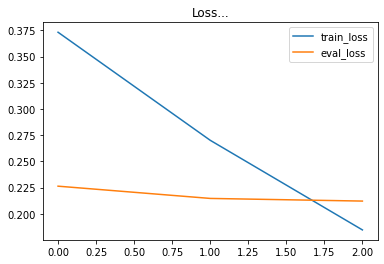
\includegraphics[width= 0.9\linewidth]{gambar/loss_concat_awal.png}
    \caption{Baseline loss value}
    \label{fig: loss_baseline}
  \end{center}
\end{figure}

\begin{figure}[h]
  \begin{center}
    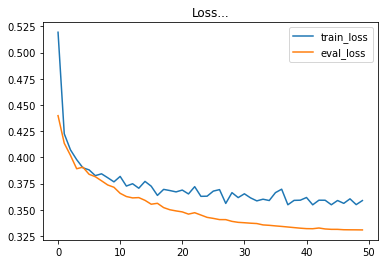
\includegraphics[width= 0.9\linewidth]{gambar/loss_freeze_50.png}
    \caption{Loss value with parameter freeze}
    \label{fig: loss_freeze}
  \end{center}
\end{figure}

\begin{figure}[h]
  \begin{center}
    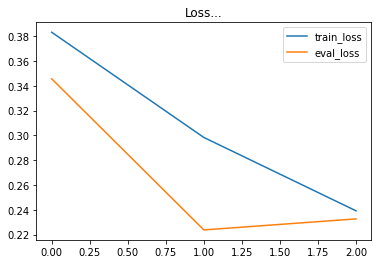
\includegraphics[width= 0.9\linewidth]{gambar/loss_dropout_new.png}
    \caption{Loss value with parameter dropout}
    \label{fig: loss_dropout}
  \end{center}
\end{figure}

According to the table \ref{tab: model_training_result}, we can safely assume that when we experiment with the parameter freeze approach, the average training time per epoch is way shorter compared to the baseline. This is most likely because the optimizer did not need to re-count all of the BERT layer's weight every epoch hence reducing the computational needs and in turn, make the training phase faster. Next, if we are comparing the loss graphic of the baseline model at figure \ref{fig: loss_baseline}, with the loss graphic of the parameter dropout approach experiment at figure \ref{fig: loss_dropout}, it can be said that the baseline graphic and by extension the model, has showing signs of overfitting, while on another side, the loss graphic looks nice with no signs of overfitting at all and all of these is achievable with a little drop in the model accuracy.